% Give an overview of PUF devices

\chapter{Physically Unclonable Functions}
\label{chapter:pufoverview}
It is desirable for a user to be sure that the device that he is using is authentic. However, due to the sophistication
of forgeries or possible communication tampering, a user might be suspicious that the system is the system it claims
to be. A device called a Physically Unclonable Function, or PUF, is a technology that remedies this problem.

A PUF device provides a unique challenge-response capability. That is, when two PUFS are provided the identical
challenge, they will each produce unique responses. In this way, a PUF, and the system it contains, 
can be identified by the response value it generates to a specific challenge. A more formalized definition of
this relationship is given below.

\begin{align*}
PUF_1(C) = R_1\\
PUF_2(C) = R_2\\
R_1 \neq R_2
\end{align*}



\section{Types of PUFs}
A PUF device provides this sort of relationship by leveraging the physical properties
of the materials in which it is instantiated. There are several different ways of doing
this, from measuring the distortions of reflected light to leveraging the
manufacturing inconsistencies from one chip to another.

Several of these are described in the remainder of this chapter, with more details
presented about the ring oscillator PUF, which is what the author typically used in
his work.

\subsection{Ring Oscillator PUF}
A Ring Oscillator PUF is a PUF design that utilizes a circuit called a Ring 
Oscillator (RO). An RO is an odd number of inverter gates tied together. Because
there are an odd number of gates, this will produce a continuously changing,
or oscillating, signal. Because it is a combination of circuits, the RO PUF can
be instantiated on a piece of silicon, such as an FPGA or ASIC device.

\begin{figure}[h] % The h specifies to place the figure 'here' as in, inline with the source code
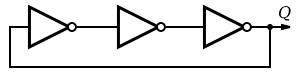
\includegraphics[]{images/ro.png}
\caption{A 3 gate Ring Oscillator}
\label{fig:ro}
\end{figure}

Depending on the number of inverter gates being used
as well as the propagation delay of every individual inverter, the output
frequency of one RO may be different from another RO. In Figure ~\ref{fig:ro},
this output signal corresponds to the signal marked $Q$.

When used as part of a PUF, the unique behaviour of an RO will be examined.
Consider again the 3 stage RO as shown in Figure \ref{fig:ro}. All three
inverter gates are assumed to have the same propagation delay and the
interconnecting wires are assumed to impose a negligible delay. However, in
an actual instantiation of an RO, these assumptions are invalid. All three inverters
should have the same propagation delay, but, due to uncontrollable manufacturing
inconsistencies and tolerances, they do not. In a similar vein, the interconnecting
wires will also impose a non-zero delay time in signal propagation. Both of these
factors will combine so that even if two ROs are produced on the same 
manufacturing line, they will generate a slightly different output frequency.

The slightly different output frequencies of two ring oscillators forms the basis
of randomness for the Ring Oscillator PUF. Because the output frequencies of the
ROs cannot be predicted, their actual frequency at runtime gives a way to uniquely
identify the individual PUF that contains them. In Figure \ref{fig:ropuf}, a more
detailed diagram of a PUF based off of ring oscillators is presented.

\begin{figure}[h]
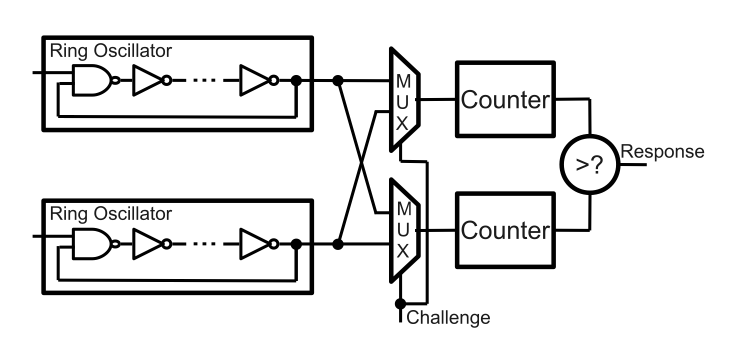
\includegraphics[width=500px]{images/ropuf.png}
\caption{A 1-bit Ring Oscillator PUF}
\label{fig:ropuf}
\end{figure}

The ring oscillator PUF shown above uses a challenge bit and feeds it to a multiplexer.
If the challenge bit is zero, the top ring oscillator will be fed to the top counter and
the bottom ring oscillator to the bottom counter. If the challenge bit is one, the top
ring oscillator will be fed to the bottom counter and the bottom ring oscillator will
be fed to the top counter. The counters will then be executed for a given amount of time.
At the expiration of this time duration, the values of the counters are compared. If the
top counter has a larger total, a zero is output as the response. If the bottom counter
has a larger total, a one is output as the response.

That is the most basic design of an RO PUF. In practice, this design is somewhat 
inefficient, since for an N-bit PUF, 2*N ring oscillators are needed, which is fairly
expensive. There has been work done for alternative designs of
an RO PUF to reduce the number of ring oscillators needed ~\cite{aegis_pool}. 
Typically, this involves using
a pool of ring oscillators and then using a multi-bit challenge to select some permutation
of them. Details presented in ~\cite{aegis_pool} illustrate that 35 oscillators can
be used to generate 133-bits of output by using this pool strategy.

\subsection{Butterfly PUF}
Another design of a PUF is called a Butterfly PUF. This design is similar to the previous
RO design in that it can be instantiated on a piece of silicon. This allows for easy
incorporation into existing FPGA designs or through the production of a custom ASIC chip.



\subsection{Optical PUF}

\subsection{Coating PUF}


\section{PUF Error and Error Correction}
An important part to consider for any PUF device is the stability of its output for
the same input. If the PUF device yields different outputs for the same challenge, the
utility of a PUF is greatly reduced. As such, it is important to examine and investigate
the stability and error rates of PUF. As the author worked primarily with RO PUFs, unless
otherwise noted, this section refers to RO PUFs.

The basic use case that should be examined is when a PUF is executed twice in the same
environment; that is, temperature, humidty, and other environmental factors are constant.
For the RO PUF design in Figure \ref{fig:ropuf}, error rates can be reduced by increasing
the time that the ring oscillators are executed. In this way, the faster ring oscillator's
counter will clearly dominate the slower ring oscillator's counter. If the execution time
is very brief, start-up times and routing delays may impose a noticeable difference and
induce additional error. Note that when the author refers to increasing timer execution
time, he is discussing orders of milliseconds. The ring oscillators were typically run
at upwards of 100 MHz, so several milliseconds was enough time for frequency differences
to become apparent.

% temperature
A source of error that can be introduced is a change in temperature. Circuits will run 
either faster or slower as temperature changes, due to the changing resistance of the
internal components. Note that this is not a behaviour specific to PUFs, but electronics
in general. As such, it is important to consider the effect of temperature on PUF devices.
Work in ~\cite{puftemp} presents detailed, empirical studies of temperature's effect on
PUFs.

% supply voltage variation

% aging
Circuit aging is another source of error that can potentially affect PUFs. Over time,
certain pathways and routes of the PUF may change in their propagation delay. Since the
PUF is predicated upon the same routes being used over and over, this can cause drastic
problems for the PUF. At the least, aging can make a PUF more susceptible to other
sources of error, but at worst case, it could cause enough bits of the PUF to change
from their original values so that the PUF is no longer identifiable as the original PUF.
Interested readers are referred to work in ~\cite{pufaging} 
which discusses PUF aging in greater detail.

% Discuss typical PUF error hamming distance

\subsection{Error Correction}
As previously described, there are multiple different factors that can affect PUFs
and their execution. If these are not mitigated, the functionality and utility of a PUF
is greatly reduced. As such, an error correction scheme is typically needed when employing
a PUF device.

Usually, the raw PUF response is not directly output, but rather, is fed into an
error correction block. The error correction block processes the raw PUF output and
removes any small errors that may be apparent and outputs the corrected response.
This is diagrammed in Figure \ref{fig:pufecc}. While it is possible to do the error
correction on a discrete chip separate from the PUF itself, it is safer to perform the
error correction on the same chip as the PUF. This prevents an adversary from potentially
intercepting the raw PUF output as it is transmitted to the error correction block. Note
that in Figure \ref{fig:pufecc}, there is a notation that the PUF and the error correction
are self contained to illustrate this.

\begin{figure}[h]
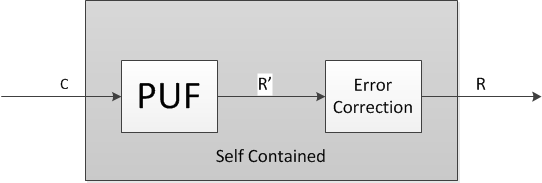
\includegraphics[]{images/puf_ecc.png}
\caption{A high level concept of PUF error correction}
\label{fig:pufecc}
\end{figure}

The author has typically employed the use of Reed-Solomon (RS) error correction codes to do 
error correction. By adding $t$ RS symbols, up to $t$ bit errors can be detected, 
while $t/2$ bit errors can actually be corrected. This is a fairly large amount of
errors to correct. For a ring oscillator PUF, \cite{pufhammingdistance} found that inter-chip
variation (that is, the same challenge) in response was approximately 0.86\%.

\section{Vulnerabilities}
% Differential power analysis (security engineering, chapter 15)

% Tampering

% Supply chain corruption

\section{Comparison to Alternatives}

\subsection{Trusted Platform Module}

\subsection{Radio Frequency Identification Tags}

